\documentclass{beamer}
%
% Choose how your presentation looks.
%
% For more themes, color themes and font themes, see:
% http://deic.uab.es/~iblanes/beamer_gallery/index_by_theme.html
%
\mode<presentation>
{
  \usetheme{Darmstadt}      % or try Darmstadt, Madrid, Warsaw, ...
  \usecolortheme{crane} % or try albatross, beaver, crane, ...
  \usefonttheme{default}  % or try serif, structurebold, ...
  \setbeamertemplate{navigation symbols}{}
  \setbeamertemplate{caption}[numbered]
  \usepackage{tikz}
  \usepackage{pgfplots}
  \usepackage{pgf}
  \usepackage{units}
  \usepackage{metalogo}
  \usepackage{graphicx}
  \usepackage{caption}
  \usepackage{subcaption}
  \usepackage[mode=buildnew]{standalone}% requires -shell-escape
  \usepgfplotslibrary{groupplots}
  \usepackage{amsmath}
} 

\usepackage[english]{babel}
\usepackage[utf8x]{inputenc}
\setbeamertemplate{footline}[frame number]

\title{Thesis Intermediate Presentation}
\author{Moritz Wolter}

\date{\today}

\begin{document}
\begin{frame}
  \titlepage
\end{frame}


% Uncomment these lines for an automatically generated outline.
\begin{frame}{Outline}
  \tableofcontents
\end{frame}

\section{Overview}
\begin{frame}{Project Overview}
	\begin{itemize}
		\item Transcribe speech utterances to characters. 
		\item Use a listen attend and spell (LAS) model to do this.
		\item Train model components jointly.
	\end{itemize}
\end{frame}



\section{Preprocessing}
\begin{frame}{Mel-Scale and Mel-Filter-Banks}
\begin{figure}
	\includestandalone[height=4 cm]{../tikz/melScale}
	\includestandalone[height=4 cm]{../tikz/melBank}
	\caption{The Mel scale and mel banks.}
	\label{fig:melBank}
\end{figure}
\end{frame}

\begin{frame}{Mel-Scale and Mel-Filter-Banks}
\begin{align}
	B(f) = 1125 ln(1 + f / 700)
\end{align}
\begin{align}
	H_m &= 0 				                       & \text{if}\;\; & k < f[m-1] \\
	H_m &= \frac{k      - f[m-1] }{f[m] - f[m-1]}  &\text{if}\;\; & f[m-1] \leq k \leq f[m] \\
	H_m &= \frac{f[m+1] - k      }{f[m + 1] - f[m]}&\text{if}\;\; & f[m] \leq k \leq f[m+1] \\
	H_m &= 0									   &\text{if}\;\; & k > f[m+1] 
\end{align}
\end{frame}

\section{Tools from Deep Learning}

\begin{frame}{Recurrent Neural Nets}
\begin{figure}
	\includestandalone[height=4 cm]{../tikz/recNet}
	\caption{Unrolling a recurrent neural net.}
\end{figure}
\end{frame}

\begin{frame}{Simple Cell}
	\begin{figure}
		\includestandalone[height=4 cm]{../tikz/recurrentCell}
		\caption{Simple recurrent cell.}
	\end{figure}
\end{frame}



\begin{frame}{Long Short Term Memory (LSTM)}
	\begin{figure}
		\includestandalone[height=6.5 cm]{../tikz/lstm}
		\caption{Visualization of the LSTM architecture}
		\label{fig:lstm}
	\end{figure}
\end{frame}

\begin{frame}{Long Short Term Memory (LSTM)}
	\begin{align}
	\mathbf{i_t} &= \sigma (\mathbf{W}_i [\mathbf{x}_t \; \mathbf{h_{t-1}} \; \mathbf{c_{t-1}}]^T + \mathbf{b}_i) \\
	\mathbf{f_t} &= \sigma (\mathbf{W}_f [\mathbf{x}_t \; \mathbf{h_{t-1}} \; \mathbf{c_{t-1}}]^T + \mathbf{b}_f) \\
	\mathbf{c_t} &= \mathbf{f}_t \mathbf{c_{t-1}} + \mathbf{i}_t \tanh( \mathbf{W}_c [\mathbf{x}_t \; \mathbf{h_{t-1}}]^T + \mathbf{b}_c ) \\
	\mathbf{o_t} &= \sigma (\mathbf{W}_o [\mathbf{x}_t \; \mathbf{h_{t-1}} \; \mathbf{c_t}]^T + \mathbf{b}_o ) \\
	\mathbf{h_t} &= \mathbf{o_t} \tanh(\mathbf{c_t})
	\end{align}
\end{frame}

\begin{frame}{Bidirectional LSTM}
	\begin{figure}
		\includestandalone[height=6.5 cm]{../tikz/blstm2}
		\caption{BLSTM architecture}
		\label{fig:blstm}
	\end{figure}
\end{frame}


\section{Listen Attend and Spell}

\begin{frame}{The LAS-Architecture}
\begin{figure}
\includestandalone[height=6.5 cm]{../tikz/lasArcBottomUp}
\caption{The LAS architecture}
\label{fig:las}
\end{figure}
\end{frame}

\begin{frame}{Listener}
\begin{itemize}
	\item Pyramidal Bidirectional long short term memory (\textit{pBLSTM}).
	\item Pyramid structure compresses the features. 
	\item Three \textit{pBLSTM}s on top of a \textit{BLSTM} layer $\Rightarrow$ compression factor $2^3 = 8 $.
	\item Pyramidal inputs concatenate the out put from previous layers:
		  \begin{align}
		  	\mathbf{h}_i^j = \text{pBLSTM}(\mathbf{h}_{i-1}^j, [\mathbf{h}_{2i}^{j-1}, \mathbf{h}_{2i+1}^{j-1}])
		  \end{align}
	\item $i$ denotes the time step (from $0$) and $j$ the layer.
\end{itemize}
\end{frame}

\begin{frame}{Attend and Spell}
\begin{itemize}
	\item attention based \textit{LSTM} transducer.
	\item Find the most likely character given the features and previously found letter-probabilities.
		  \begin{align}
			\mathbf{c}_i &= \text{AttentionContext}(\mathbf{s}_i,\mathbf{H}) \\
			\mathbf{s}_i &= \text{RNN}(\mathbf{s}_{i-1},\mathbf{y}_{i-1},\mathbf{c}_{i-1}) \\
			P(\mathbf{y}_i|\mathbf{x},y_{<i}) &= \text{CharacterDistribution}(\mathbf{s}_i,\mathbf{c}_{i})
		  \end{align}

\end{itemize}
\end{frame}
\begin{frame}{Attention Context}
	\begin{itemize}
		\item Produce a context vector $\mathbf{c}_i$, with alignment information.
			  \begin{align}
			  	e_{i,u} &= \phi(\mathbf{s}_i)^T \psi(\mathbf{h}_u) \\
			  	\alpha_{i,u} &= \frac{\exp(e_{i,u})}{\sum_u exp(e_{i,u})} \\
			  	\mathbf{c}_i &= \sum\limits_{u} \alpha_{i,u}\mathbf{h}_u 
			  \end{align}
		\item $\phi$ and $\psi$ are feed-forward MLP networks.
		\item $\mathbf{s}_i$ is the decoder state.
		\item The $\alpha$s work like a sliding window.
		\item $U$ denotes the total number of feature vectors.
	\end{itemize}
\end{frame}

\begin{frame}{Decoding and Rescoring}
\begin{itemize}
	\item Humans do not read character distributions.
	\item Left to right beam search turns distributions into text.
	\item Generate a tree using the $n$ most likely characters.
	\item Select from the tree according to:
		\begin{align}
		s(\mathbf{y}|\mathbf{x}) = \frac{\log P(\mathbf{y}|\mathbf{x})}{ |\mathbf{y}|_c} + \lambda \log P_{LM}(\mathbf{y})
		\end{align}
	\item The first summand is the total probability found from the tree. 
	\item The second summand is a weighted language model contribution.
\end{itemize}
\end{frame}



\begin{frame}{What is Tensorflow?}
	\begin{itemize}
		\item \textquotedblleft TensorFlow is an interface for expressing machine learning algoritms and an implementation for executing such algorithms. \textquotedblright \footnote{TensorFlow:
			  Large-Scale Machine Learning on Heterogeneous Distributed Systems, Abadi et al, Google Research.}
		\item Computations are described by directed graphs. 
		\item Data-Tensors flow along graph edges.
		\item Graphs are constructed using user specified elementary
			  operations.
		\item Computations are started by requesting certain values, which leads
			  to (partial) evaluation of the graph.
	\end{itemize}
\end{frame}


\begin{frame}{Tensorflow}
\begin{figure}
\centering
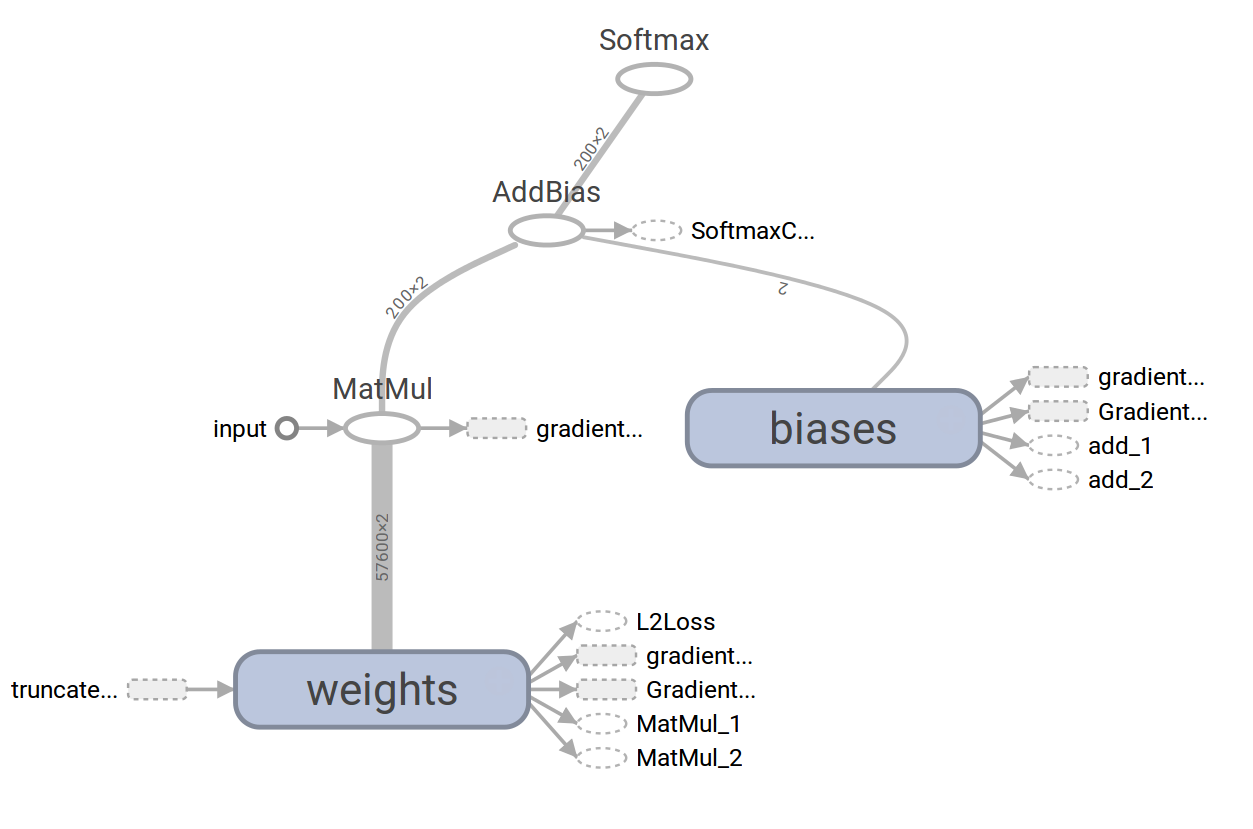
\includegraphics[width=0.7\linewidth]{../png/net1}
\caption{A simple linear node in tensorboard}
\label{fig:net1}
\end{figure}
\end{frame}

\section{Planning}
\begin{frame}{What happend so far? What will happen next?}
\begin{itemize}
\item What happend so far?
	\begin{enumerate}
		\item Literature overview.
		\item Learned how to use tensorflow.
		\item Looked into timit and aurora4.
	\end{enumerate}
\item What will happen next?
		\begin{enumerate}
			\item Finish implementing a skeleton LAS on Timit. 
			\item Decoding with beam search.
			\item Port to aurora4.
		\end{enumerate}
\end{itemize}
\end{frame}


\section{Questions}
\begin{frame}{Summary and Questions}
	The presentation covered:
	\begin{itemize}
		\item Input feature generation.
		\item The LSTM building block.
		\item A LAS-Architecture overview.
		\item The tensorflow toolbox.
		\item The plan.
	\end{itemize}
	Thank you for your attention. Questions? \\
	\texttt{moritzalexander.wolter@student.kuleuven.be}
\end{frame}


\end{document}
